\documentclass[12pt,oneside,a4paper]{article}   
\usepackage[czech, english]{babel}
\usepackage{amsmath}
\usepackage{epsf,epic,eepic,eepicemu,url}
\usepackage[utf8]{inputenc}
\usepackage{graphicx}
\newenvironment{listing}
{\begin{list}{}{\setlength{\leftmargin}{1em}}\item\scriptsize\bfseries}
{\end{list}}

\begin{document}
\begin{center}
\bf Semestralní projekt MI-PAR 2010/2011:\\[5mm]
    Paralelní řešení úlohy MBG - Minimální obarvení grafu\\[5mm]
       Jiří Špaček (spaceji3@fit.cvut.cz)\\
       Matěj Plch (plchmate@fit.cvut.cz)\\[2mm]
magisterské studium, FIT ČVUT, Kolejní 550/2, 160 00 Praha 6\\[2mm]
9.\,12.\,2010
\end{center}

\section{Definice problému}
Cílem této práce je navrhnout a implementovat paralelní algoritmus pro hledání minimálního uzlového obarvení souvislého k-regulárního grafu zadaného pomocí jeho matíce sousednosti. Vstupem algoritmu je tedy graf $G(V,E)$, kde $V$ je množina uzlů, $E$ je množina hran, $n = |V|$ je počet uzlů grafu a $k$ je stupeň uzlů grafu. Pro graf musí být splněna podmínka $n >= k >= 3$ a navíc musí být alespoň jedno z $n$ a $k$ sudé.

Uzlové obarvení grafu $G(V,E)$ definujeme jako zobrazení $B: V \rightarrow N$, pro které platí, že pro libovolné 2 uzly $u, v \in V$, které jsou spojeny hranou $(u, v) \in E$ platí $B(u) \neq B(v)$.  Takovému obarvení říkáme minimální pokud neexistuje menší počet barev, kterými jsme schopni takto graf obarvit. Tomuto počtu říkame chromatické číslo grafu a značíme jej $\chi(G)$.

Výstupem programu je hodnota chromatického čísla následovaná vstupní maticí sousednosti, která má na hlavní diagonále hodnoty nejlepšího nalezeného obarvení. Těsná spodní mez algoritmu nastává pro 2 barvy v případě, že $G$ je bipartitní. Triviální horní mez pro počet barev je $b = k + 1$.

\section{Popis sekvenčního algoritmu}
Sekvenční algoritmus funguje na principu prohledávání stavového prostoru do hloubky (Depth-first search)s použitím zásobníku. Stavy jsou realizovány jako trojice hodnot: (index uzlu, barva uzlu, nejvyšší dosavadní obarvení). Jako implementace zásobníku bylo zvoleno pole s dynamickou velikosti realizované konntejnerem vector dodávaným v knihovně STL. 

Pseudokód algoritmu:
\begin{listing}
\begin{verbatim}

function SeqSolver(graph) begin

    colors = EmptyArray;
    stack = EmptyStack;

    chroma_num = graph.NodesDegree + 1;

    push(stack, State(0,1,1));

    while (stack is NOT empty) do

        state = pop(stack));
        colors[state.index] = state.color;
        Fill(colors, state.index+1, NO_COLOR);
        
        if(state.index == graph.NodesCount+1) then
            
            if(state.maxColor <= optimal) then
                optimal = state.maxColor;
                solution = colors;
            endif

        endif

        if(state.color >= optimal) then
            continue; // BACKTRACK!
        endif
        
        newState = State(state.index+1, maxColor);
       
        for( newColor = optimal; newColor >= 1, newColor++ ) do
            if( IsAllowedColoring(newState, newColor) ) then
                newState.color = newColor;
                push(stack, newState);
            endif
         endfor

    endwhile

    return (optimal, colors); 
end
\end{verbatim}
\end{listing}

\section{Popis paralelního algoritmu}

Paralelní algoritmus je typu G-PBB-DFS-D

Jako algoritmus pro hledání dárce byl zvolen pro svoji jednoduchost algoritmus asynchroních cyklických žádostí (ACZ-AHD) s lokálním čítačem potencionálních dárců udržovaným v proměnné \texttt{mNeighbour}.

Jistým specifikem našeho řešení je způsob jakým řídíme odchozí zprávy. Pokud v nějakém bodě výpočtu nastane událost, na kterou je potřeba zareagovat odesláním zprávy jinému pracujícímu procesoru (třeba v případě kdy je nalezeno nové optimálnější řešení a je potřeba o tomto řešení informovat i ostatní procesory nebo v případě kdy je vyprázdněn zásobník a je žádáno o novou práci), je jako reakce na tuto událost vygenerován token typu \texttt{OutgoingMsg}, ktery je umísten do fronty odchozích zpráv \texttt{mOutgoingQueue}. Ta je pak následně procházena odbavována v metodě \texttt{ProcessOutgoingMessages}. Toto řešení bylo zvoleno z důvodu oddělení části obsluhující příchozí komunikaci, části obsluhující odchozí komunikaci a části starající se o vlastní výpočet. Diky tomu, že je \texttt{mOutgoingQueue} implementována jako fronta, nemůže dojít k předbíhání odchozích zpráv.


Hlavní smyčka stavového stroje obsahuje obsahuje celkem 3 části. 

První částí je obsluha příchozích zpráv (metoda \texttt{ProcessIncomingMessages}). Pokud se stavový stroj nachází v aktivním stavu (tj. provádí se výpočet nad daty), je fornat příchozích zpráv kontrolována v pravidelných intervalech definovaných konstantou \texttt{CHECK\_MSG\_AMOUNT}. Pokaždé když dosáhne čítač expandovaných stavů násobku této hodnoty provede se tělo metody \texttt{ProcessIncomingMessages}.

V druhé části hlavní smyčky je prováděna expanze nových stavů na zásobníku a tedy i vlastní výpočet. Tato část programu je identická s implementací sekvenčního algoritmu. Pokud je během vykonávání vyprázdněn zásobník přejde stavový stroj do pasivního stavu (\texttt{PASSIVE}) a zároveň je do fronty odchozích zpráv umístěna žádost o novou práci. 

Na závěr každé iterace je zavolána metoda \texttt{ProcessOutgoingMessages}, která prochází frontu odchozích požadavků a generuje odchozí MPI komunikaci.

Pseudokód hlavní smyčky:
\begin{listing}
\begin{verbatim}
function main_loop() begin
    while (nejsme ve stavu FINISHED) do
        work_counter++;
        if ((work_counter % CHECK_MSG_AMOUNT) == 0)  then
            Zpracuj_příchozí_zprávy();   // ProcessIncomingMessages();
        endif

        if (Zásobník NENÍ prázdný)  then
            Expanduj_nové_stavy();
        endif
    
        if (Zásobník_JE_prázdný && jsme ve stavu ACTIVE) then
            přidat_do_odchozí_fronty(NO_WORK);
            stav = WAITING_FOR_WORK;
        endif
    
        Zpracuj_odchozí_zprávy();   // ProcessOutgoingMessages();
    endwhile
end

\end{verbatim}
\end{listing}


\section{Měření paralelního zrychlení algoritmu}
	Pro ověření správné funkčnosti a efektivity algoritmu byla provedena série měření na třech náhodně vygenerovaných instancích. Pro tyto instance byly naměřeny sekvněční časy měření, které následně slouží k výpočtu paralelního zrychlení algroitmu. Sekvenční časy jsou uvedeny v následující tabulce. 


\subsubsection*{Měření času sekvenčního algoritmu}
\begin{center}
  \begin{tabular}{| c || c | c | c | c | c | c | }
    \hline
       & \multicolumn{3}{|c|}{\bf Měřené instance}  \\ \hline
       & \bf 40n16k & \bf 38n16k & \bf 30n19k \\ \hline
   \bf Sekv. čas &  299  & 612 & 1257 \\ 
    \hline
  \end{tabular}
\end{center}


\subsection*{Měřené instance}
\subsubsection*{Instance 1}
\begin{center}
  \begin{tabular}{| l | l | }
    \hline
    \bf Identifikátor & 40n16k \\ \hline
    \bf Počet uzlů & 40 \\ \hline
    \bf Stupeň uzlů & 16 \\ \hline
    \bf Sekv. čas &  299 sek. (4 min. 59 sek.) \\ 
    \hline
  \end{tabular}
\end{center}


\subsubsection*{Instance 2}
\begin{center}
  \begin{tabular}{| l | l | }
    \hline
    \bf Identifikátor & 38n16k \\ \hline
    \bf Počet uzlů & 38 \\ \hline
    \bf Stupeň uzlů & 16 \\ \hline
    \bf Sekv. čas &  612 sek. (10 min. 12 sek.) \\ 
    \hline
  \end{tabular}
\end{center}


\subsubsection*{Instance 3}
\begin{center}
  \begin{tabular}{| l | l | }
    \hline
    \bf Identifikátor & 30n19k \\ \hline
    \bf Počet uzlů & 30 \\ \hline
    \bf Stupeň uzlů & 19 \\ \hline
    \bf Sekv. čas &  1257 sek. (20 min. 57 sek.) \\ 
    \hline
  \end{tabular}
\end{center}

\newpage

\subsection*{Měření paralelního zrychlení}
Paralelní zrychlení $S(n,p)$ je definováno jako $S(n,p) = \frac{SU(n)}{T(n,p)}$. Byly provedeny celkem 3 série měření, vždy se stejnými instancemi grafů a na stejných počtech paralelních jader. 

\subsubsection*{Měření paralelního algoritmu 1}
\begin{center}
  \begin{tabular}{| c || c | c | c | c | c | c | }
    \hline
      & \multicolumn{6}{|c|}{\bf Měřené instance}  \\ \hline
     \bf Typ sítě & \multicolumn{2}{|c|}{\bf 40n16k} & \multicolumn{2}{|c|}{\bf 38n16k} & \multicolumn{2}{|c|}{\bf 30n19k} \\ \hline
    \bf p & \bf eth & \bf infi & \bf eth & \bf infi & \bf eth  & \bf infi \\ \hline \hline
   \bf 2 & 226.532 & 228.25 & 466.363 & 441.935 & 1014.4 & 1029.87 \\ \hline
   \bf 4 & 129.275 & 127.274 & 221.7 & 220.617 & 532.689 & 515.5 \\ \hline
   \bf 8 & 624.141 & 621.929 & 275.906 & 272.638 & 894.993 & 889.235 \\ \hline
   \bf 16 & 78.4224 & 102.012 & 144.314 & 140.983 & timed out & timed out \\ \hline
   \bf 24 & 364.806 & 357.089 & 175.519 & 171.921 & 179.296 & 169.727 \\ \hline
   \bf 32 & 77.865 & 83.0722 & 116.981 & 122.94 & 1403.13 & 1387.25 \\
    \hline
  \end{tabular}
\end{center}

\begin{figure}[ht]
\begin{minipage}[b]{0.5\linewidth}
\centering
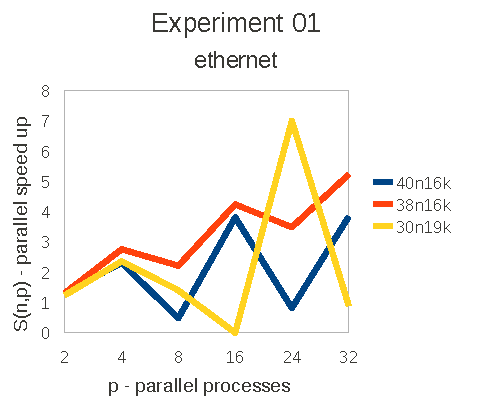
\includegraphics[scale=0.9]{img/par-ex01-eth.pdf}
\caption{Graf $S(n,p)$ - síť ethernet}
\label{fig:figure1}
\end{minipage}
\hspace{0.5cm}
\begin{minipage}[b]{0.5\linewidth}
\centering
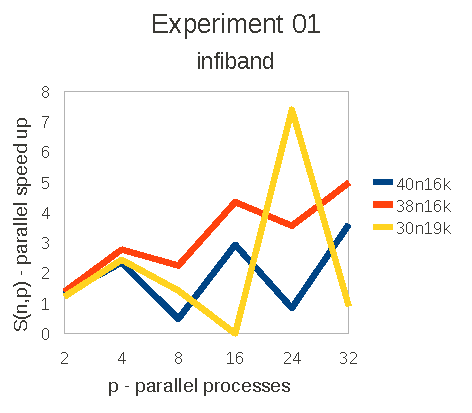
\includegraphics[scale=0.9]{img/par-ex01-infi.pdf}
\caption{Graf $S(n,p)$ - síť infiband}
\label{fig:figure2}
\end{minipage}
\end{figure}

\newpage 

\subsubsection*{Měření paralelního algoritmu 2}
\begin{center}
  \begin{tabular}{| c || c | c | c | c | c | c | }
    \hline
      & \multicolumn{6}{|c|}{\bf Měřené instance}  \\ \hline
     \bf Typ sítě & \multicolumn{2}{|c|}{\bf 40n16k} & \multicolumn{2}{|c|}{\bf 38n16k} & \multicolumn{2}{|c|}{\bf 30n19k} \\ \hline
    \bf p & \bf eth & \bf infi & \bf eth & \bf infi & \bf eth  & \bf infi \\ \hline \hline
   \bf 2 &232.886 & 228.14 & 442.596 & 451.81 & 1016.35 & 1030.15 \\ \hline
   \bf 4 & 128.932 & 128.248 & 223.016 & 222.086 & 521.393 & 511.338 \\ \hline
   \bf 8 & 625.043 & 619.248 & 273.075 & 272.316 & 896.574 & 876.985 \\ \hline
   \bf 16 & 168.254 & 166.218 & 143.589 & 138.877 & timed out & timed out \\ \hline
   \bf 24 & 361.318 & 356.171 & 175.071 & 171.302 & 175.835 & 175.97 \\ \hline
   \bf 32 & 89.1364 & 74.7474 & 144.826 & 118.823 & 1398.09 & 1507.82 \\
    \hline
  \end{tabular}
\end{center}

\begin{figure}[ht]
\begin{minipage}[b]{0.5\linewidth}
\centering
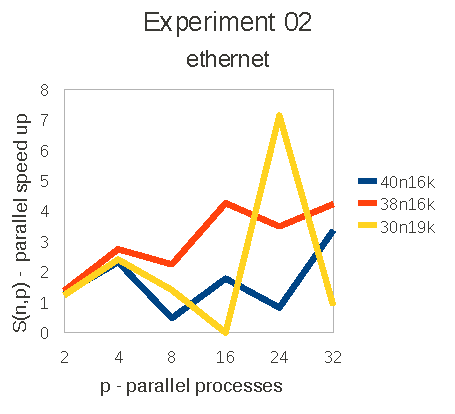
\includegraphics[scale=0.9]{img/par-ex02-eth.pdf}
\caption{Graf $S(n,p)$ - síť ethernet}
\label{fig:figure1}
\end{minipage}
\hspace{0.5cm}
\begin{minipage}[b]{0.5\linewidth}
\centering
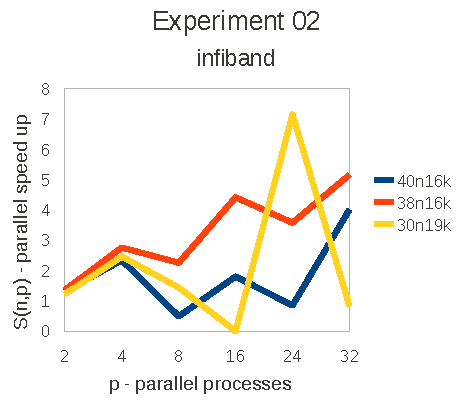
\includegraphics[scale=0.9]{img/par-ex02-infi.pdf}
\caption{Graf $S(n,p)$ - síť infiband}
\label{fig:figure2}
\end{minipage}
\end{figure}

\newpage

\subsubsection*{Měření paralelního algoritmu 3}
\begin{center}
  \begin{tabular}{| c || c | c | c | c | c | c | }
    \hline
      & \multicolumn{6}{|c|}{\bf Měřené instance}  \\ \hline
     \bf Typ sítě & \multicolumn{2}{|c|}{\bf 40n16k} & \multicolumn{2}{|c|}{\bf 38n16k} & \multicolumn{2}{|c|}{\bf 30n19k} \\ \hline
    \bf p & \bf eth & \bf infi & \bf eth & \bf infi & \bf eth  & \bf infi \\ \hline \hline
   \bf 2 & 228.582 & 233.059 & 442.052 & 446.74 & 1039.03 & 1060.1 \\ \hline
   \bf 4 & 129.986 & 129.982 & 227.458 & 222.934 & 521.737 & 522.717 \\ \hline
   \bf 8 & 623.891 & 625.484 & 273.851 & 275.803 & 885.468 & 892.308 \\ \hline
   \bf 16 & 168.542 & 165.002 & 143.137 & 140.363 & timed out & timed out \\ \hline
   \bf 24 & 362.389 & 355.877 & 176.748 & 166.969 & 418.786 & 171.088 \\ \hline
   \bf 32 & 74.7078 & 70.9551 & 115.58 & 118.701 & 1409.76 & 1375.41 \\
    \hline
  \end{tabular}
\end{center}

\begin{figure}[ht]
\begin{minipage}[b]{0.5\linewidth}
\centering
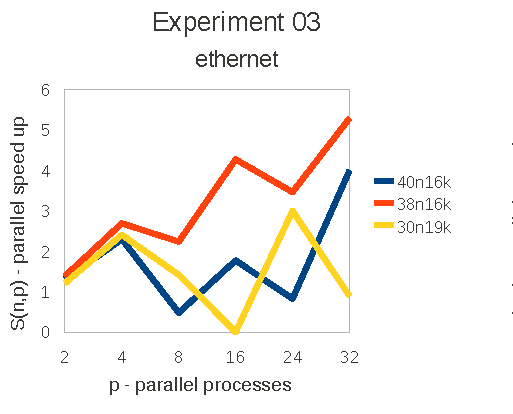
\includegraphics[scale=0.9]{img/par-ex03-eth.pdf}
\caption{Graf $S(n,p)$ - síť ethernet}
\label{fig:figure1}
\end{minipage}
\hspace{0.5cm}
\begin{minipage}[b]{0.5\linewidth}
\centering
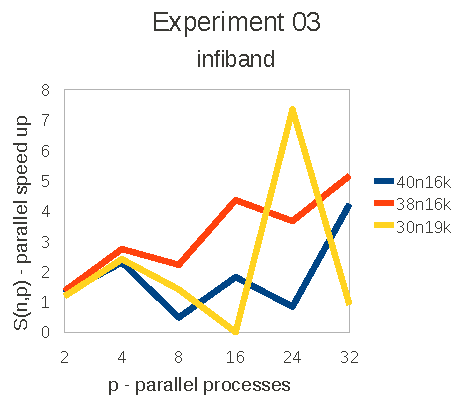
\includegraphics[scale=0.9]{img/par-ex03-infi.pdf}
\caption{Graf $S(n,p)$ - síť infiband}
\label{fig:figure2}
\end{minipage}
\end{figure}

\subsection*{Zhodnocení výsledků měření}
Z naměřených dat je na první pohled patrné, že délka běhu výpočtů v síti ethernet se téměř neliší od doby běhu v síti Infiband (řádově jednotky sekund). To ovšem není očekávaný stav, protože síť Infiband by měla být řádově rychlejší než ethernet. Tento výsledek lze vysvětlit relativně střídmým používáním síťové komunikace a hlavně přenášením velmi malých objemů dat po síti (větší datový tok je generován pouze jednou na začátku výpočtu při distribuci počátečních dat mezi jádra).

Stejně tak se nějak význačně neliší doby běhu instancí neliší opakované experimenty se stejnou instancí na stejném počtu jader, což ukazuje vždy stejné dělení práce mezi jednotlivá jádra a tím i stejné výpočetní doby.

To co nás však u tohoto měření zajímá nejvíce je zda bylo dosaženo nějakého zrychlení oproti sekvenčnímu algoritmu. Z výše uvedených grafů je zřejmé, že k lineárnímu zrychlení zcela evidentně nedošlo. Dokonce pro některé instance spuštěných na určitých počtech jader trvá výpočet déle než sekvenční algoritmus spuštěný na jediném procesoru. V případě instance s identifikátorem 30n19k spuštěném na 16ti jádrech je toto zpoždění tak velké, že dochází k překročení časového limitu 2400 sekund (40 minut). Tyto výsledky jsou bohužel znakem závažné chyby v implementaci paralelního algoritmu, kterou se nám přes všechno úsilí nepodařilo odladit.

Při ladění algoritmu jsme se zaměřili zejména na různá nastavení algoritmu, mezi které patří nastavení konstanty \texttt{CHECK\_MSG\_AMOUNT} udávající frekvenci kontroly fronty příchozích zpráv a nastavení limitu odmítnutých požadavků o práci (\texttt{mRefusedWorkReqs}), při jehož překročení přechází procesor do pasivního stavu a čeká na ukončovacího peška.

Nejpravděpodobnějším vysvětlením poklesu výkonu bude zřejmě chybná implementace algoritmu pro dynamické vyvažování zátěže a komunikace s tímto spojená. Jako možná protiopatření, která se v tomto případě nabízí můžeme zvolit například jiný způsob dělení zásobníku. Z důvodů nedostatku času a vytíženosti testovacího prostředí se nám toto nepodařio ověřit.

Dalším možným vysvětlením proč k takovému zpoždění dochází může být problém s rozesíláním nově nalezených optimálních řešeních problému. Pokud toto nefunguje, může nastat situace, kdy některá jádra prohledávají daleko větší statové prostory než je potřeba. Tato funkčnost však byla důkladně otestována a nebyla v ní nalezena žádná chyba.

Zajímavým faktem který lze z naměřených dat napozorovat je téměř lineární zrychlení, které dosahují všechny instance 2 a 4 procesory. Zda se v tomto případě jedná pouze o náhodu, či zda to svědčí o správné funkci algoritmu na těchto počtech jader bohužel nelze z tak malého počtu měřených instancí jednoznačně určit.

\section{Závěr}
Při psaní této práce jsme získali cenné zkušeností s návrhem jednoduchých aplikací určených pro paralelní zpracování. V průběhu vývoje aplikace v zásadě nedošlo k významějším problémům, za což lze vděčit zejména knihovně MPI, řešících velké množství nízkoúrovňových záležitostí za programátora. Přesto však výsledný algoritmus nefungoval ani zdaleka ne optimálně a pro jeho zdárné odladění by bylo nutné provádět jeho měření na daleko větším počtu testovacích instancí, na což bohužel není testovací prostředí připraveno. 

\section{Literatura}
\begin{itemize}
\item Pavel Tvrdík - Paralelní systémy a algoritmy
\item Josef Kolář - Teoretick8 informatika
\item Michal Šoch - Programování pod MPI
\end{itemize}


\renewcommand{\refname}{Literatura}
\bibliographystyle{ieeetr}
{
 \bibliography{refs}
}


\end{document}
